\zotelo{../thesis.bib}

\chapter{Introduction}
\label{chap:intro}

A lot of astrophysics has to do with observing objects at various radiation
frequencies. Many objects are sources of high energy radiation, including but
not limited to pulsars, gamma-ray bursts, magnetars, super-massive black holes,
etc. In many of the objects, the spectrum is highly non-thermal, and the
radiation is produced by accelerated particles. The study of particle
acceleration and dissipation of other forms of energy into particle kinetic
energy is therefore vital in the study of high-energy astrophysics.

In many of the sources, the most notable source of energy for nonthermal
particles is the magnetic energy. In some sources such as pulsars, magnetic
field plays an intermediary role, acting as a channel that converts the
rotational energy of the pulsar ultimately into the particle energy, which then
is radiated away and produce the observed radio/X-ray/gamma ray emission. In
other sources such as magnetars it is the magnetic energy itself that is
directly converted to particle energy that is radiated.

% TODO: Go into more details, and mention past work
The dissipation of magnetic energy and acceleration of particles is a highly
nonlinear process, and very difficult to model directly. In the past people have
tried different methods. Some attempt to model the whole system by treating the
plasma as fluid, and use magnetohydrodynamics or force-free approximation. Some
isolate part of the system and study the detailed local evolution of
eletromagnetic fields. It is only recently that computational power has
increased to the level that we could attempt a first-principle direct simulation
of the system of interest.

This dissertation will be focusing on the physics of isolated neutron stars. In
the following sections we will examine the history and basic physics of
rotation-powered pulsars, and the exotic magnetars which have extremely high
magnetic field. Finally we will outline the chapters of the thesis.

\section{Pulsars}
\label{sec:intro-pulsars}

\subsection{Early Observations}

The first observational discovery of the rotation-powered pulsars (RPP) dates
back to late 1960s \citep{hewish_observation_1968}. In this paper a periodic
radio source was reported to be emitting regular pulsation at a frequency of
$81.5\,\mathrm{MHz}$, with a period of $1.337\,\mathrm{s}$ at extreme accuracy.
The pulse width of the object gives an upper bound on its physical size, which
should not exceed $4.8\times 10^3\,\mathrm{km}$. The extreme constancy of the
intrinsic period suggests that the source is a massive object, rather than some
astrophysical plasma configuration. It was therefore conjectured that this
pulsed radio emission was coming from a compact star: a white dwarf or a neutron
star; the extreme regular pulsation is a result of its rapid rotation
\citep{gold_rotating_1968}.

\begin{figure}[h]
  \centering
  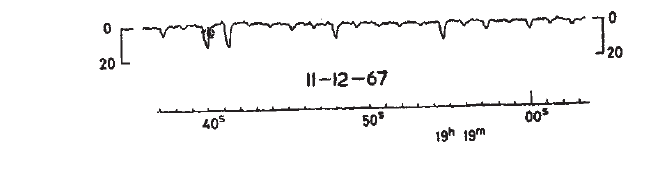
\includegraphics[width=0.6\textwidth]{pics/intro/pulses.png}
  \caption{A record of the pulsating radio source discovered in 1967
    \citep{hewish_observation_1968}}
  \label{fig:pulse}
\end{figure}

More pulsars were soon discovered, e.g.\ the Vela with a period of
$89\,\mathrm{ms}$ \citep{large_pulsar_1968} and the Crab with a period of
$33\,\mathrm{ms}$ \citep{lovelace_pulsar_1968}. Slowing down of the periods were
also discovered in the known pulsars. The spin-down luminosity can be easily
estimated given the period and period derivative of the pulsar:
\begin{equation}
  \label{eq:spindown-power}
  L_{d} = -I\Omega\dot{\Omega} = 4\pi^2 I\frac{\dot{P}}{P^3}
\end{equation}
which works out to be $\sim 10^{39}\,\mathrm{erg/s}$ for the Crab pulsar, which
has $P = 33\,\mathrm{ms}$ and $\dot{P} = 4.2\times 10^{-13}\,{s\;s^{-1}}$. This
matches the observed luminosity of the Crab nebula, and a model was soon
proposed by \citet{gold_rotating_1969} that gas was liberated from the star and
accelerated to relativistic energies, forming a corotating magnetosphere around
the star up to the radius where corotation speed becomes equal to the speed of
light, $R_\mathrm{LC} = c/\Omega$. This radius is called the light-cylinder
radius. In this model, the relativistic gas carry away most of the spin-down
luminosity, and make its contribution to the luminosity of the nebula.

The spin-down of the pulsar was typically modeled by a spinning magnetic dipole
in vacuum. A magnetic dipole of strength $\mu$ will lose energy at a rate:
\begin{equation}
  \label{eq:dipole-spin-down}
  L_{d} = \frac{2}{3}\frac{\mu^2\Omega^4}{c^3}
\end{equation}
therefore one can naively estimate the surface magnetic field by equating this
with the spin-down luminosity \eqref{eq:spindown-power}
\begin{equation}
  \label{eq:surface-B-field}
  B_0 = 3.2\times 10^{19}\sqrt{P \dot{P}}\,\mathrm{G}
\end{equation}

For typical pulsar parameters, this gives a polar magnetic field of the order
$\sim 10^{12}\,\mathrm{G}$. The strong magnetic field required rules out the
possibility of a white dwarf, and since then a rapid rotating neutron star has
been the standard model for a rotation-powered pulsar. Equation
\eqref{eq:surface-B-field} remains the standard formula for estimating the surface
magnetic field of a newly discovered pulsar.

\subsection{High-energy radiation from pulsars}
\label{sec:observ-high-energy}

Although radio emission has been the primary wavelength at which rotation
powered pulsars are studied, only a tiny fraction ($\sim 10^{-5}$) of their
spin-down power actually goes into radio emission. For young pulsars and
millisecond pulsar (MSPs), a significant fraction of their spin-down power go
into gamma-rays in the $100\,\mathrm{MeV}$--$30\,\mathrm{GeV}$ band \citep[see
e.g.][]{abdo_fermi_2010}.

\begin{figure}[h]
  \centering
  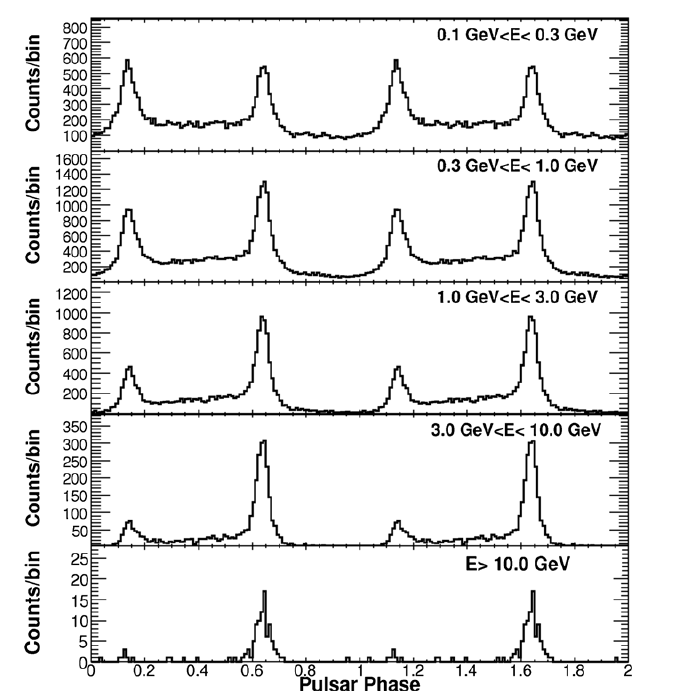
\includegraphics[width=0.7\textwidth]{pics/intro/geminga2.png}
  \caption{Gamma-ray lightcurves of Geminga in five energy ranges, from {\it
      Fermi} observations \citep{abdo_fermi-lat_2010}.}
  \label{fig:geminga}
\end{figure}

Take the pulsar Geminga for example. It is the second brightest non-variable
$\mathrm{GeV}$ gamma-ray source in the sky. Its gamma-ray emission was first
discovered in the 70s by the SAS-2 satellite
\citep{fichtel_high-energy_1975,kniffen_distribution_1975}. In contrast to the
Crab pulsar, Geminga is observed to be radio quiet, and is the first
representative of the class of radio quiet gamma-ray pulsars. As can be seen
from figure \ref{fig:geminga}, the gamma-ray peak comes in pairs in every
period, in contrast to the typical radio peaks in rotation powered pulsars,
suggesting that the gamma-ray emission comes from very different region than
the radio emission.

After the launch of the {\it Fermi} satellite, the catalog of gamma-ray pulsars
exploded from 7 to well over 130 \citep{abdo_first_2010,abdo_second_2013}. The
gamma-ray pulsars are evenly divided into 3 groups: millisecond pulsars, young
radio-loud pulsars, and young radio-quiet pulsars. This discovery revolutionized
the way pulsars were studied. The pulsed gamma-ray emission typically carries
the highest fraction of the spin-down power $L_{d}$, therefore it can reveal the
most information about the particle acceleration and field structure in pulsar
magnetospheres, much more so than the radio emission.

Many pulsars are also found to be X-ray sources, with pulsations detected in
many of them. The emission is usually made up of two components: a thermal
component from surface cooling or heated polar caps, and a non-thermal component
that is most likely magnetospheric \citep{kaspi_isolated_2006}.


% The biggest difficulty in pulsar modeling is to account for this broadband
% radiation. A self-consistent model needs to explain not only the

\subsection{Theoretical models of the pulsar magnetosphere}
\label{sec:intro-pulsar-theory}

Despite the success of a simple vacuum dipole model, it proves to be extremely
difficult to make a more detailed self-consistent model. The vacuum dipole
model has a few problems. First is that, the electric field from
uni-polar induction effect gives a voltage that can accelerate particles to
% TODO: how high voltage?
This voltage has two effects: it exceeds the binding energy of electrons and
ions at the surface of the neutron star and can extract charged particles from
the stellar surface, and it also accelerates the
extracted particles to energies that produce high-energy photons that are
capable of interacting with the intense magnetic field and convert into
$e^{\pm}$ pairs, thus inducing a pair cascade \citep{erber_high-energy_1966}.

As a result, it is not possible for the pulsar magnetosphere to be near vacuum.
A minimum corotating charge density is guaranteed around the pulsar which is
conventionally called the Goldreich-Julian density \citep{goldreich_pulsar_1969}:
\begin{equation}
  \label{eq:gj-density}
  \rho_\mathrm{GJ} = -\frac{\bOm\cdot \mathbf{B}}{2\pi c}\frac{1}{1 - (\Omega r/c)^2\sin^{2}\theta}
\end{equation}
where $\theta$ is the angle between magnetic axis and the rotation axis.

The problem of the Goldreich-Julian model is that charge lifted from the
surface alone is not sufficient to fill the magnetosphere with
$\rho_\mathrm{GJ}$. For an aligned rotator (magnetic axis aligned with rotation
axis), there exists an electrostatic equilibrium solution for the lifted charge
\citep{jackson_new_1976, krause-polstorff_pulsar_1985,
  krause-polstorff_electrosphere_1985}. The surface charge are lifted to form a
dome around the poles of the star, and a torus near the equator. In both the
dome and the torus $\mathbf{E}\cdot \mathbf{B} = 0$, whereas an unscreened
vacuum gap exists between them (figure \ref{fig:electrosphere-intro}). This
equilibrium solution has no outgoing Poynting flux, therefore no spin-down at
all. It is a dead pulsar.

\begin{figure}[h]
  \centering
  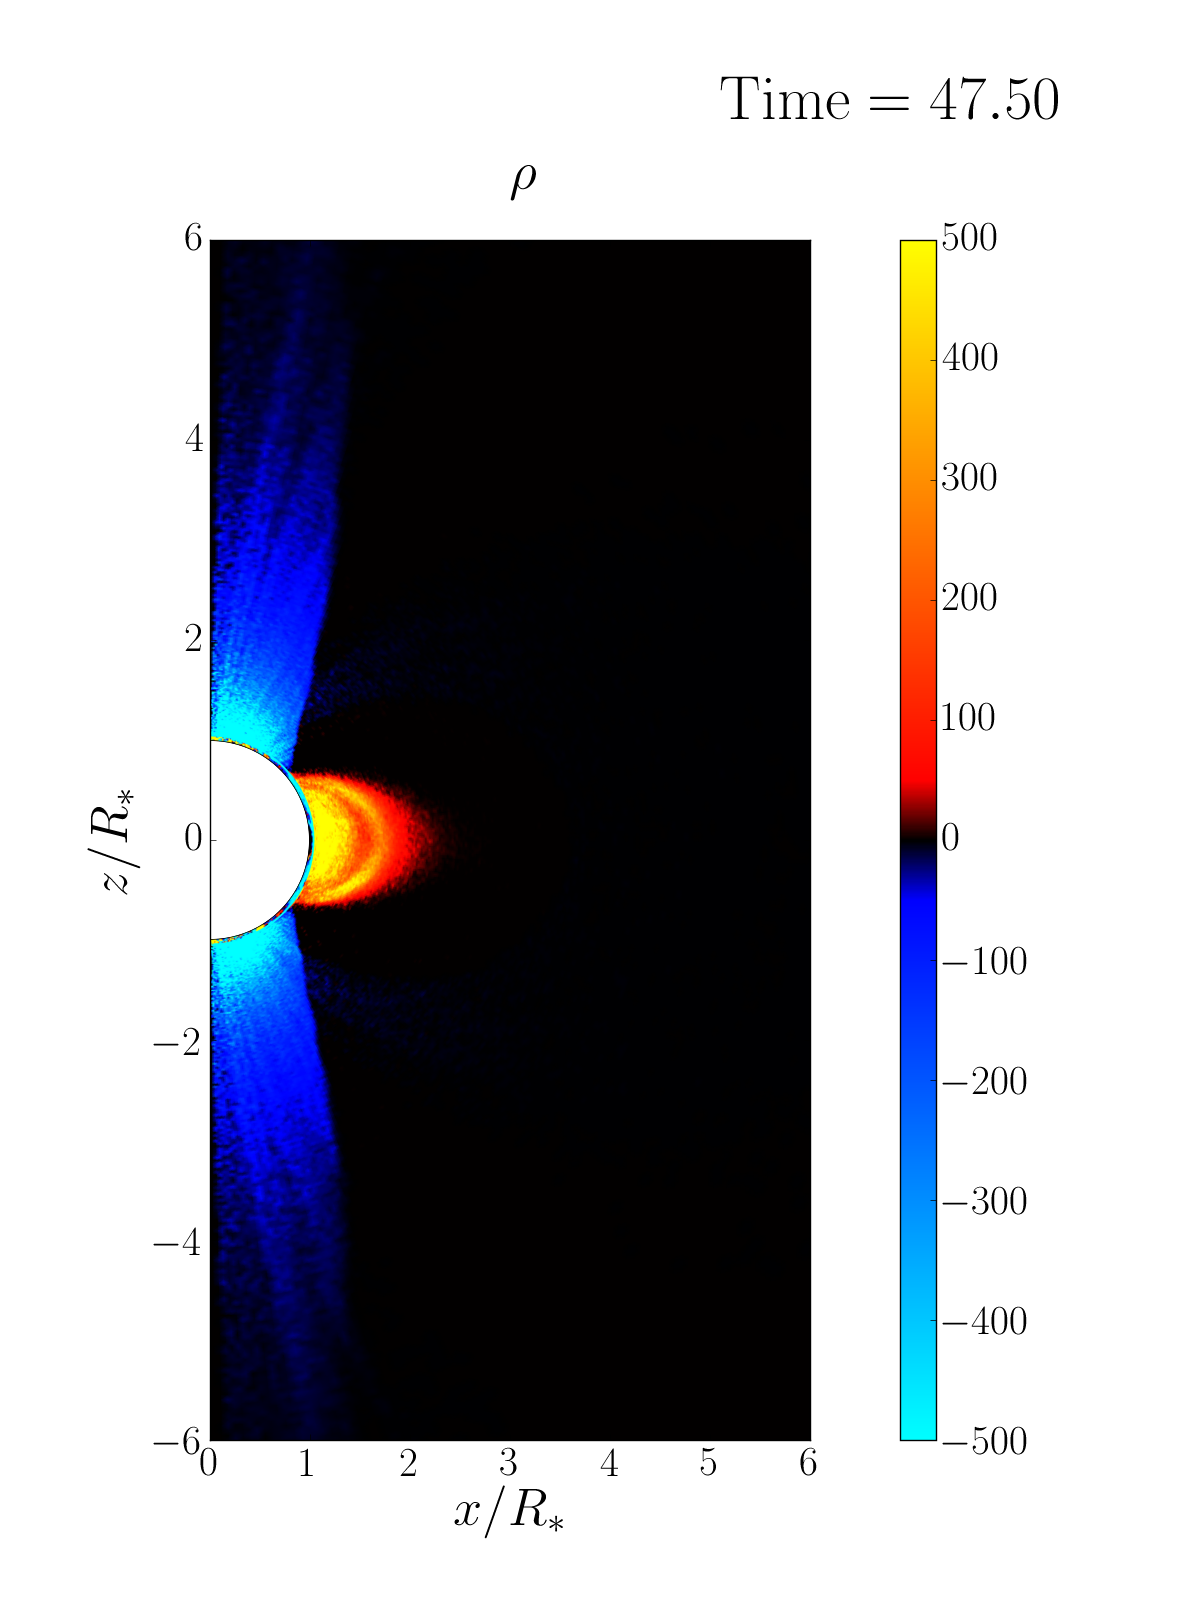
\includegraphics[width=0.6\textwidth]{pics/intro/electrosphere-new.png}
  \caption{Charge density distribution of the electrosphere of an aligned
    rotator. Blue indicates negative charge and red indicates positive charge.}
  \label{fig:electrosphere-intro}
\end{figure}

It was speculated by \citet{spitkovsky_electrodynamics_2004} that oblique
rotators will be able to escape this fate due to diocotron instability
developing inside the torus, which leads to its slow expansion and eventually
reaching the light cylinder. This might jump-start the global current
circulation and allow the pulsar to start operating. But no simulation or
analytical results has been able to confirm this hypothesis. Furthermore,
\citet{petri_relativistic_2007} showed that this instability is suppressed by
relativistic effects that become important near the light cylinder.

Another problem with the electrosphere is that, a huge unscreened gap exists
between the dome and torus, capable of accelerating stray particles to very high
energies. These particles will be able to produce curvature photons that are
able to interact with the magnetic field to produce $e^{\pm}$ pairs. This
eventually renders the electrosphere solution unstable to pair creation.
Chapter \ref{chap:pulsar} will study the global pulsar magnetosphere, motivated
by the study of the polar cap particle acceleration.

Chapter \ref{chap:magnetar} will study the twisted magnetosphere of magnetars.

% Local Variables:
% TeX-master: "../thesis"
% zotero-collection: #("16" 0 2 (name "Thesis"))
% End:
